%%%%%%%%%%%%%%%%%%%%%%%%%%%%%%%%%%%%%%%%%%%%%%%%%%%%%%%%%%%%%%%%%%%%%%%%%%%%%%%%%%%%%%%%
% Criação de Fluxograma usando LaTeX
%
% Assunto: escrever aqui um comentário com uma
%          breve explicação do exercício
%
% Autores:
%     Guilherme Miranda Lustosa Cantarelli
%     Luiza Saraiva peixoto costa
%     Anderson nunes
%
% Coordenação:
%     Prof. Dr. Ruben Carlo Benante
%
% Data: 2024-04-25
%%%%%%%%%%%%%%%%%%%%%%%%%%%%%%%%%%%%%%%%%%%%%%%%%%%%%%%%%%%%%%%%%%%%%%%%%%%%%%%%%%%%%%%%


%%%%%%%%%%%%%%%%%%%%%%%%%%%%%%%%%%%%%%%%%%%%%%%%%%%%%%%%%%%%%%%%%%%%%%%%%%%%%%%%%%%%%%%%
\documentclass{article}
\usepackage{tikz}
\usetikzlibrary{shapes.geometric, arrows}

\tikzstyle{startstop} = [rectangle, rounded corners, minimum width=3cm, minimum height=1cm,text centered, draw=black, fill=red!30]
\tikzstyle{process} = [rectangle, minimum width=3cm, minimum height=1cm, text centered, draw=black, fill=orange!30]
\tikzstyle{decision} = [diamond, minimum width=3cm, minimum height=1cm, text centered, draw=black, fill=green!30]
\tikzstyle{arrow} = [thick,->,>=stealth]

\begin{document}

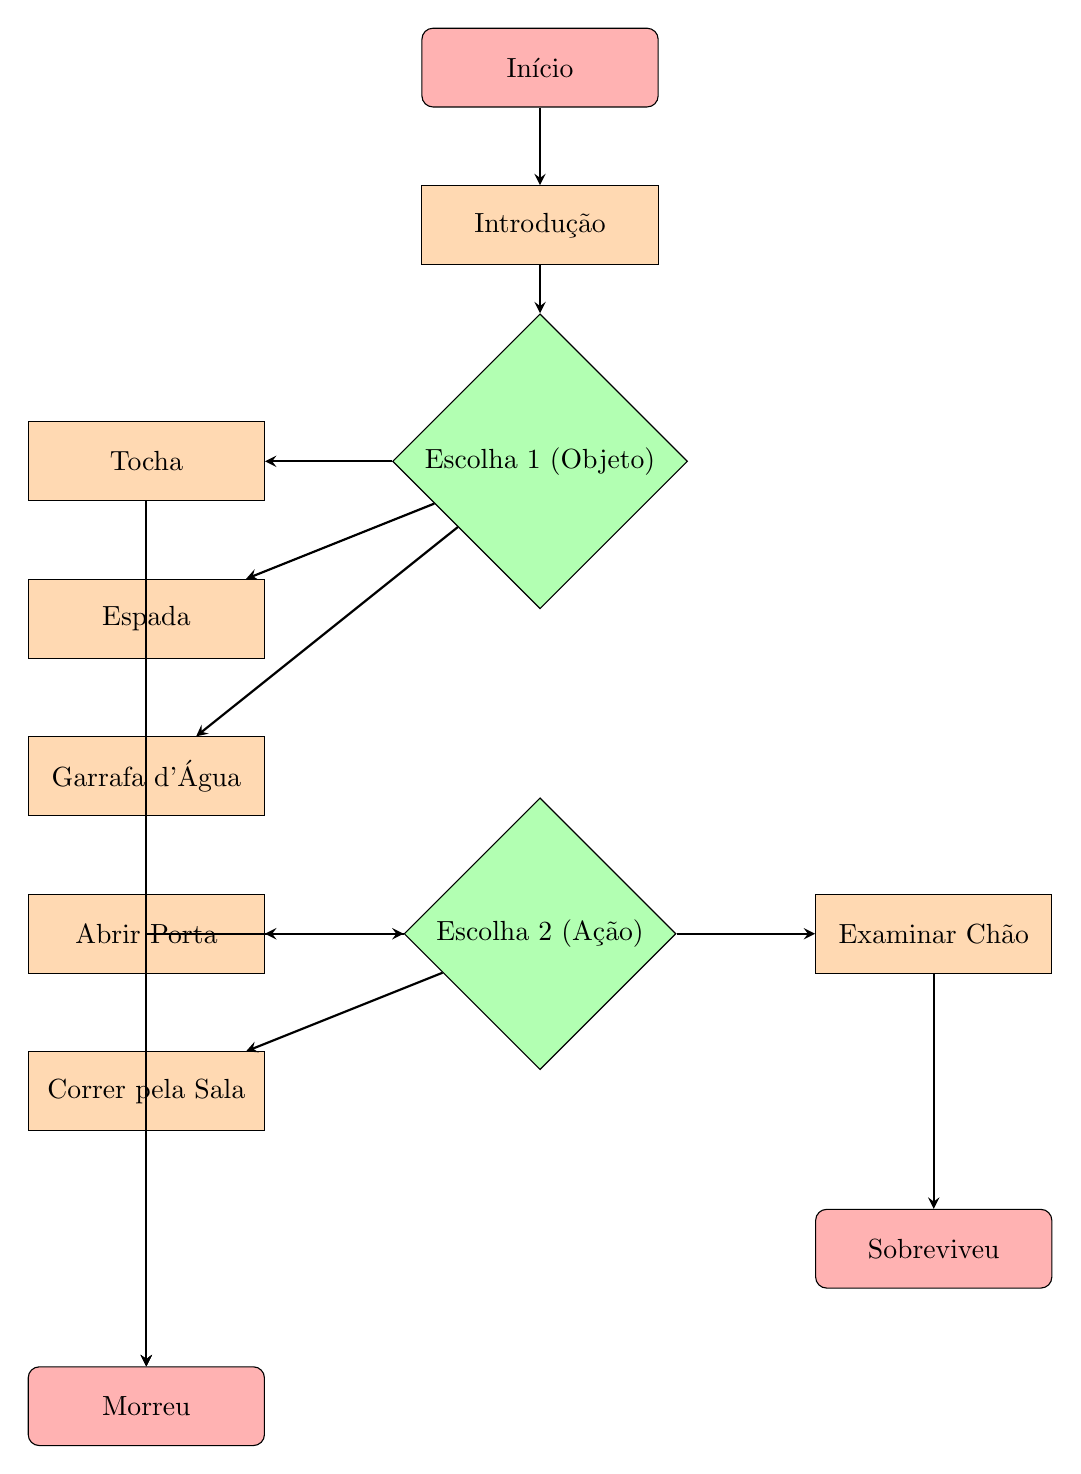
\begin{tikzpicture}[node distance=2cm]

    % Nodes
    \node (start) [startstop] {Início};
    \node (intro) [process, below of=start] {Introdução};
    \node (choice1) [decision, below of=intro, yshift=-1cm] {Escolha 1 (Objeto)};
    \node (torch) [process, left of=choice1, xshift=-3cm] {Tocha};
    \node (sword) [process, below of=torch] {Espada};
    \node (water) [process, below of=sword] {Garrafa d'Água};
    \node (choice2) [decision, below of=choice1, yshift=-4cm] {Escolha 2 (Ação)};
    \node (open) [process, left of=choice2, xshift=-3cm] {Abrir Porta};
    \node (examine) [process, right of=choice2, xshift=3cm] {Examinar Chão};
    \node (run) [process, below of=open] {Correr pela Sala};
    \node (survive) [startstop, below of=examine, yshift=-2cm] {Sobreviveu};
    \node (death) [startstop, below of=run, yshift=-2cm] {Morreu};

    % Arrows
    \draw [arrow] (start) -- (intro);
    \draw [arrow] (intro) -- (choice1);
    \draw [arrow] (choice1) -- (torch);
    \draw [arrow] (choice1) -- (sword);
    \draw [arrow] (choice1) -- (water);
    \draw [arrow] (torch) |- (choice2);
    \draw [arrow] (sword) -- (death);
    \draw [arrow] (water) -- (death);
    \draw [arrow] (choice2) -- (open);
    \draw [arrow] (choice2) -- (examine);
    \draw [arrow] (choice2) -- (run);
    \draw [arrow] (open) -- (death);
    \draw [arrow] (run) -- (death);
    \draw [arrow] (examine) -- (survive);

\end{tikzpicture}

\end{document}
